\section{Introduction}

As part of the NSF-supported NDN ``Next Phase'' research from 2014-2016, 
the NDN project team has selected two network environments, {\bf Open mHealth} and {\bf
Enterprise Building Automation \& Management}, and one application
cluster, {\bf Mobile Multimedia}, to drive our research, verify the
architecture design, and ground evaluation of the next phase of our project.
The two environments represent critical areas in the design space for
next-generation Health IT and Cyberphysical Systems, respectively.  They
also extend work started in the previous NDN FIA project on participatory
sensing and instrumented environments to focus on specific application
ecosystems where we believe NDN can address fundamental challenges that
are unmet by IP.  Based on the successful initial results of previous
NDN research, we have identified Mobile  Multimedia as an application
area of cross-cutting relevance, motivated not only by the
network environments above but our team's desire to further develop
NDN by using it for our everyday communication.

This technical report provides background information on the {\bf Open mHealth}
network environment including key application challenges faced using
IP and describes the design for a pilot application that the NDN team is 
building.  It serves as the primary design document for this application. 

\subsection{Open mHealth Background}

%\begin{figure*}
%\begin{center}
\begin{wrapfigure}{r}{0.5\textwidth}
%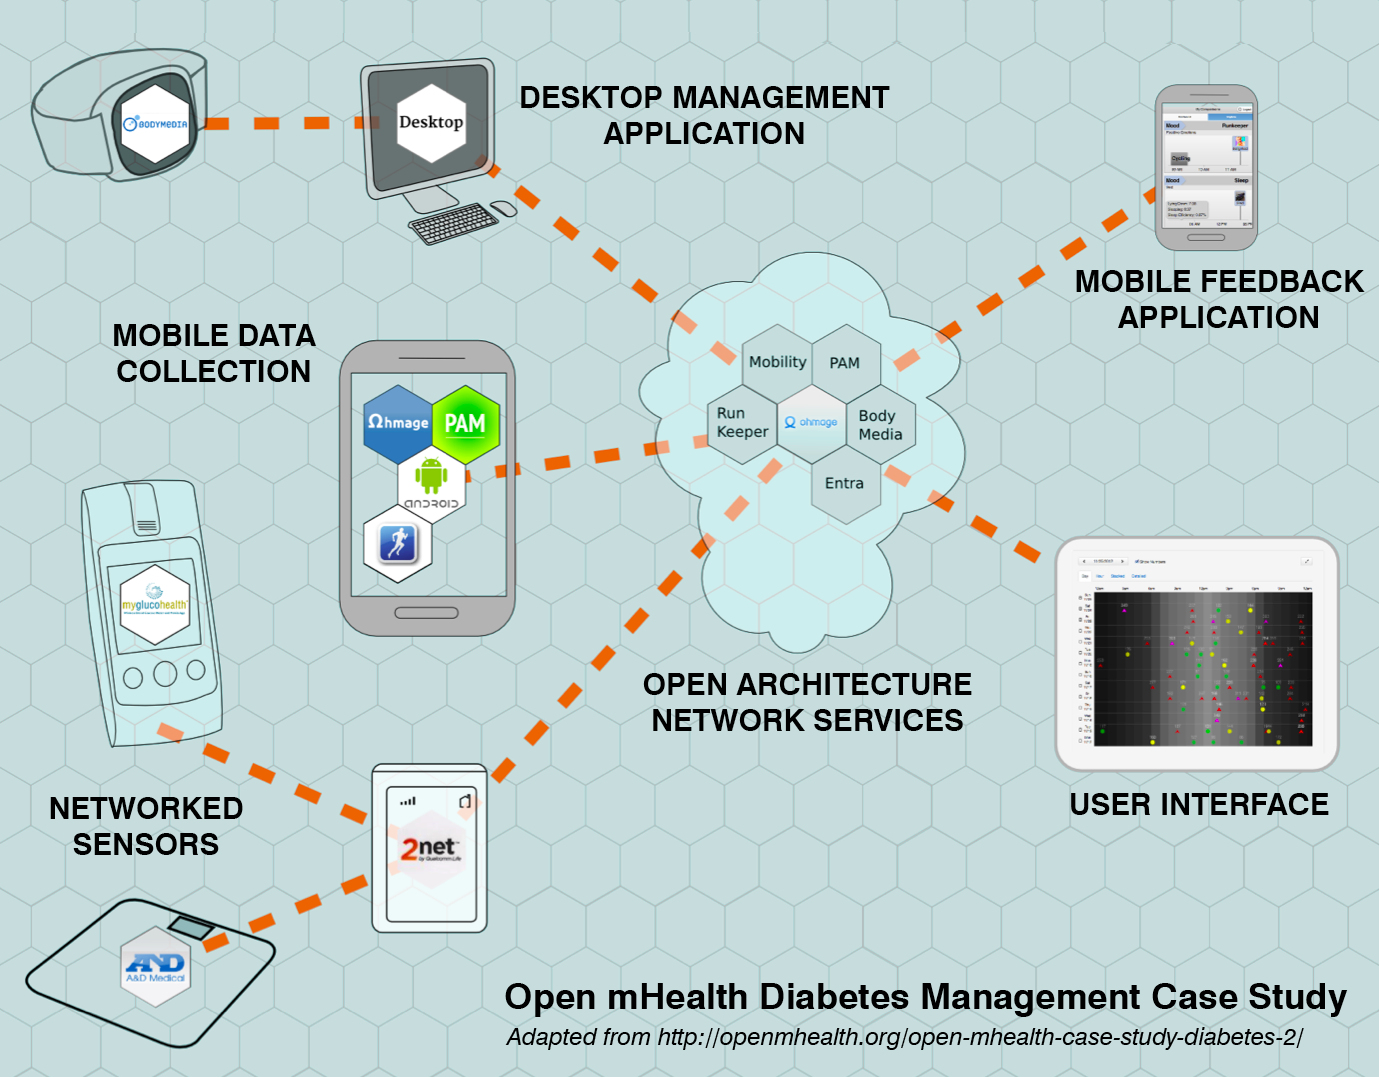
\epsfig{file=figures/OpenmHealth-figure.eps,width=.48\textwidth}
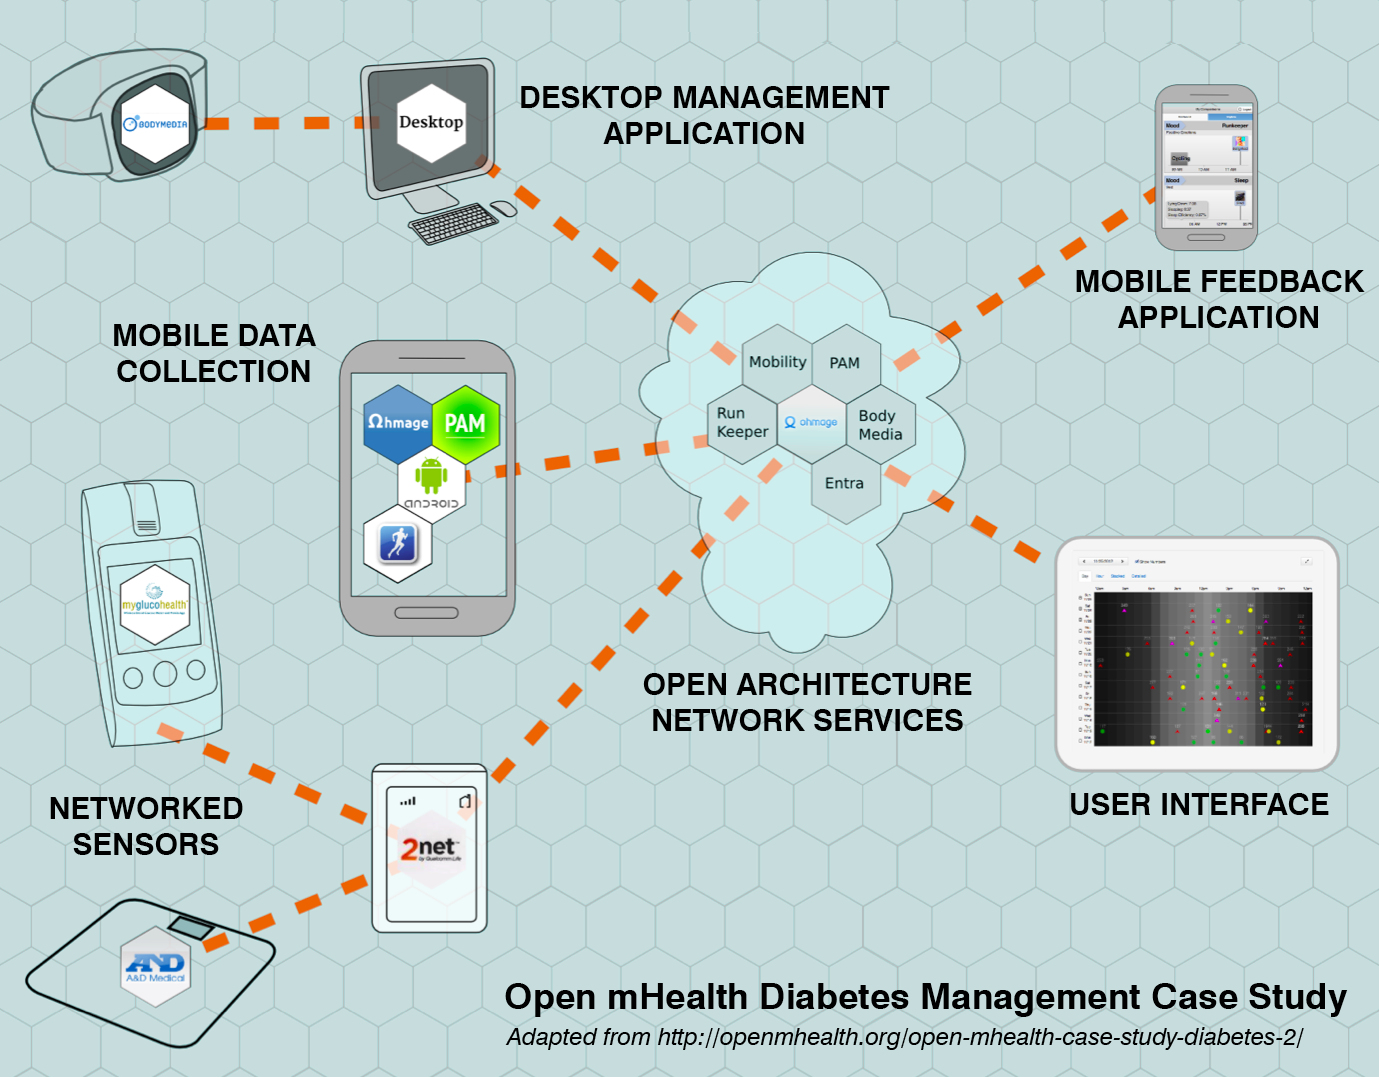
\includegraphics[width=.5\textwidth]{figures/OpenmHealth-figure}
\vskip -5pt
\caption{Networked data producers and consumers in a diabetes management case study from the Open mHealth team, who promote interoperability between mobile health components via community-standardized data exchange.~\cite{SimEstrin2010}}
\vskip 6pt
\label{fig:mHealth}
\end{wrapfigure}
%\end{center}
%\end{figure*}

Mobile health (mHealth) has emerged as both an important commercial
market and a key area of Health IT, a national priority. The 2013 mHealth
Summit
%\footnote{\url{http://www.mhealthsummit.org/about-summit/overview}} 
will host over 4,500 participants.  Recent surveys suggest there are
over 13,000 health-related apps available to Apple iPhone
users, and over 6000 for Android users~\cite{Eng_Lee13}.  The 
Internet's role as a critical enabler of mHealth will grow further over
the next decade.

Mobile health continues our work in the first NSF-supported NDN project
on participatory sensing. 
To explore mHealth as a network environment for NDN, our team will
collaborate with the Open mHealth project~\cite{chen2012making}  led by
Deborah Estrin (Cornell) and Ida Sim (UC San Francisco). Within the many
applications of mobile technology to health, Open mHealth focuses on
leveraging the public's everyday mobile devices (cell phones, tablets,
etc.)~to extend evidence-based interventions beyond the reach of traditional
care and thereby improve disease management and prevention.  For
example, mobile applications exist or have been proposed to manage:
pre- and post-natal care of mothers~\cite{Gurman_etal12}; 
diabetes~\cite{Sieverdes_etal13,Tamrat_Kachnowski12}; 
everyday activity in stroke patients and others with chronic
disease~\cite{Dobkin_Dorsch11}; and community exposure to
environmental pollutants~\cite{Ramanathan20114481}.



The Open mHealth team envisions that the Internet will interconnect 1)
data capture, 2) secure storage, 3) modeling and analytics, and 4) user
interface components to create a modular, layered sense-making framework.  
Such applications will use low-level state
classifications of raw data (e.g., estimated activity states such as
sitting, walking, driving from continuous accelerometer and location
traces) to derive mid-level semantic features (e.g., total number of
ambulatory minutes, number of hours spent out of house), that can 
be mapped to behavioral biomarkers for specific diseases
(e.g., chronic pain, diabetes, multiple sclerosis, fatigue, depression,
etc)~\cite{Estrin_IPSN_2013}.


For example, Figure~\ref{fig:mHealth} shows a network of open components
for self-care of diabetes, which affects 25.8M people in the U.S., 
less than half of whom meet recommended standards, such as blood
glucose index levels, for managing their own health. Type 1 diabetics
continuously self-monitor blood glucose and insulin levels, and
other important factors such as diet and exercise.  Many developers are
exploring mobile health technologies to assist self-monitoring and
diabetes management, since almost all
	%given that 85\% to 90\% of 
patients have access to
mobile health capable technology~\cite{Sieverdes_etal13}.   
	%current and envisioned 
But such applications often have proprietary or siloed
designs that inhibit data exchange, e.g., data streams from 
apps for blood glucose and physical activity do not easily
integrate,  %(especially by the patient).  This is 
a missed opportunity to
provide more comprehensive analysis and coaching to the patient and more
complete longitudinal data to providers.

The Open mHealth team instead advocates an interoperable,  Internet-inspired
approach. They propose a thin waist of open data interchange standards
that will enable an ecosystem of sensing, storage, analysis, and user
interface components to support medical
discovery and evidence-based care.  In the same way that the Internet's
IP layer enabled innovation and interoperability among distributed
devices, they believe a common and open approach to mHealth data exchange
will  encourage the emergence of a market-supported, patient-centered
landscape of innovative health applications. Central to this vision is
patient-controlled, privacy-aware data exchange across device, component,
and application boundaries.  The focus on \emph{data exchange as the
backbone of the application ecosystem} makes open mHealth an excellent
network environment to both drive and evaluate NDN.

%\begin{figure*}
%\begin{center}
\begin{wrapfigure}{r}{0.5\textwidth}
%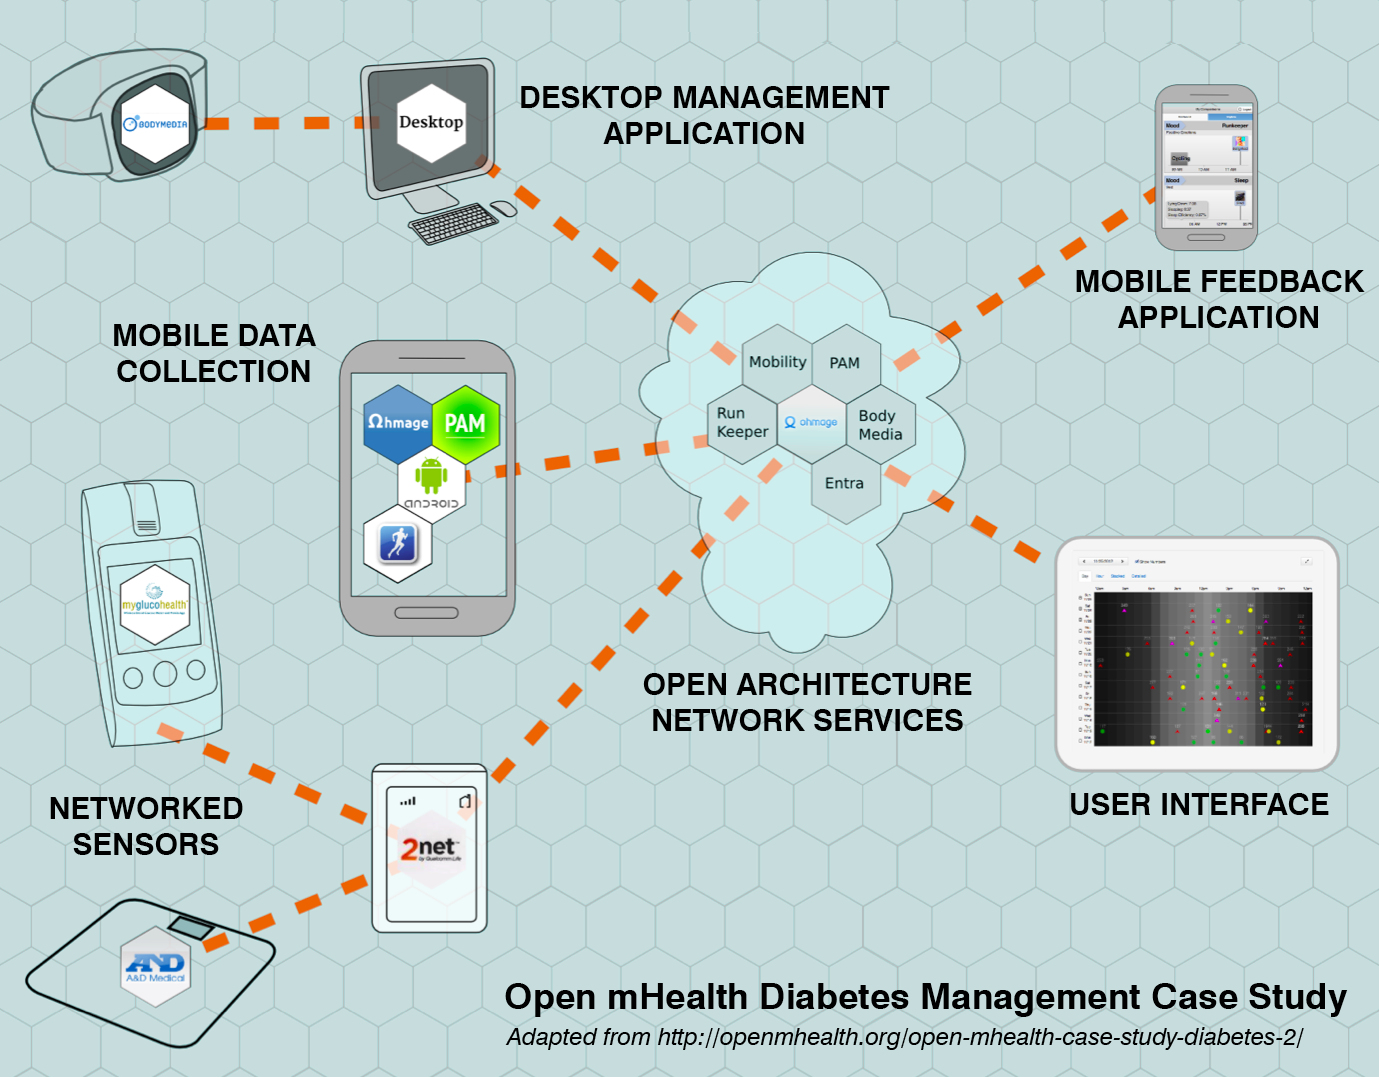
\epsfig{file=figures/OpenmHealth-figure.eps,width=.48\textwidth}
\includegraphics[width=.5\textwidth]{figures/mHealth-hourglass}
\vskip -5pt
\caption{The Open mHealth architecture uses a data-centric hourglass model, where the interoperability layer (``thin waist'') is based on standardized data exchange.~\cite{SimEstrin2010}}
\vskip 6pt
\label{fig:mHealth}
\end{wrapfigure}
%\end{center}
%\end{figure*}


\subsection{Collaboration}

We will partner with the Open mHealth team -- both its leadership and
developers -- to understand the requirements and current state-of-the-art
in this network environment, as well as limitations they face from the
current Internet architecture. We will pick one or more 
applications (e.g., diabetes management or post-heart attack health management) 
that are representative of the envisioned ecosystem, and port existing software
of the Open mHealth team to the NDN architecture.  We will use an interactive
development process, soliciting regular feedback from the Open mHealth team.   

\subsection{Proposed Milestones 2014-2016}

\begin{itemize}
\item Review limitations in current IP-based architecture for Open mHealth needs. (Y1)
\item Design namespace, repository, trust and communication model for use cases, e.g., diabetes or PTSD treatment (Y1; updated in Y2)
\item Repository implementation providing backing storage for prototype applications. (Y1)
\item Integrate named data networking into the Ohmage mobile data collection framework. (Y2)
\item Pilot user-facing application using NDN, for beta testing by Open mHealth project team. (Y2)
\end{itemize}






